\newpage
\appendix
\section{附录}
本附录给出补充实验结果与详细分析，以进一步验证我们提出的方法。具体而言，我们提供 SPAR 算法与 Clip-Forward-KL 目标的消融实验，并扩展评估事实感知 RL 框架与 Gated Eagle-3 推测解码机制。有关训练与评估所使用提示词的完整细节，请参阅对应的 \href{https://github.com/baichuan-inc/Baichuan-M3-235B/tree/main/prompts}{GitHub} 仓库。

\subsection{SPAR 的消融实验}

\begin{figure}[H]
    \centering
   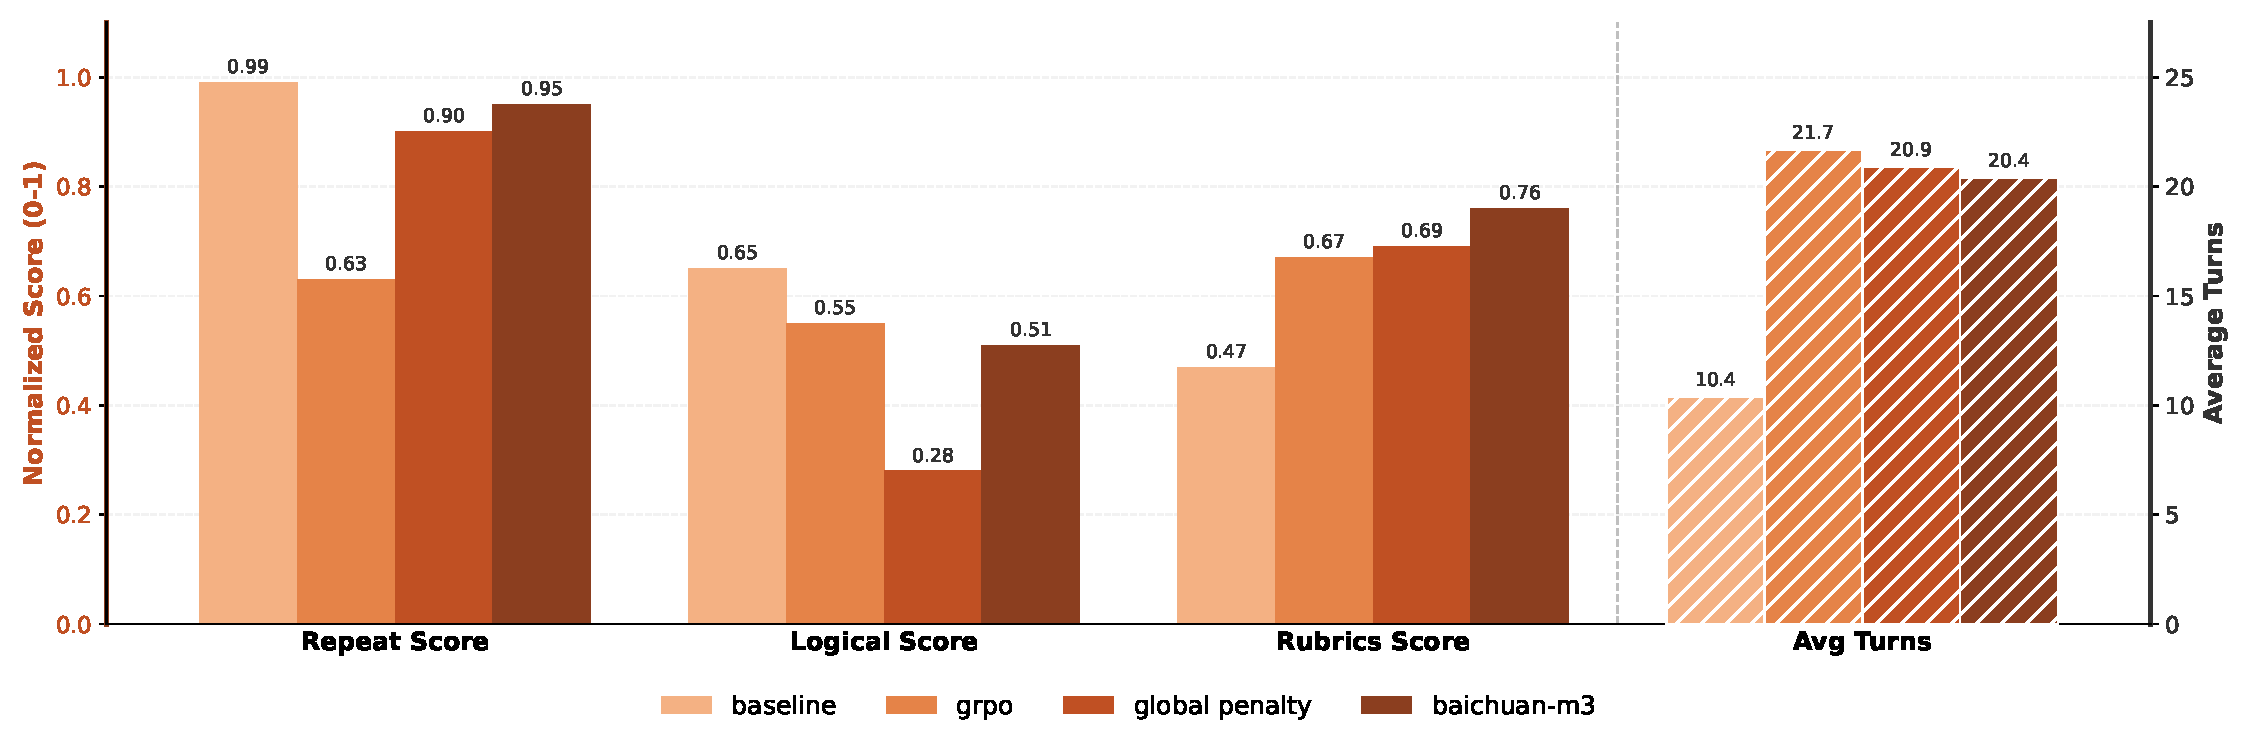
\includegraphics[width=0.98\linewidth]{image/SPAR.pdf}
    \caption{多轮医学问诊任务中 SPAR 与基线模型的性能对比。}
    \label{fig:SPAR}
\end{figure}

为系统评估 SPAR 算法在多轮医学问诊任务中的有效性，我们采用以下实验配置进行消融：
\begin{enumerate}
\item \textbf{Backbone：} 使用 Baichuan-M3 基座模型（RL 之前）作为基础架构。

\item \textbf{GRPO（全局奖励）：} 采用 GRPO 算法，仅使用基于最终问诊结果的全局奖励，不包含中间反馈。

\item \textbf{全局惩罚：} 在 GRPO 基线上引入全局重复惩罚以减轻对话冗余。

\item \textbf{SPAR（Baichuan-M3）：} 实现所提出的逐步奖励计算算法，提供细粒度指导。
\end{enumerate}

\textbf{指标：} 评估框架包含四项归一化到 $[0, 1]$ 区间的指标：重复评分（衡量非冗余）、逻辑评分、量表评分与平均轮次（Avg Turns）。其中前两项通过 GPT-5 对对话日志进行三档打分 $(0, 1, 2)$ 并归一化得到。

\textbf{结果：} 如图~\ref{fig:SPAR} 所示，仅使用全局奖励的 GRPO 训练虽能稳步提升量表评分，但也增加了冗余问询（重复评分下降）。加入全局重复惩罚可有效降低冗余，却导致逻辑评分显著下降，表明逻辑碎片化严重。这表明粗粒度全局惩罚会显著扰动模型的自然推理流程。相比之下，SPAR 取得更好的平衡：显著减少重复同时保持逻辑连贯。该双重优化使模型在有限问诊轮次中提取更高密度的关键医学信息。



\subsection{事实感知 RL} 
\subsubsection{蒸馏事实抽取模型的评估}
\label{sec:extraction_model_evaluation}

离线事实抽取以 GPT-5 作为参考抽取器，但在在线强化学习中部署如此大的教师模型在计算上不可接受。为此，我们通过监督微调（SFT）训练较小模型，以在在线 RL 中充当高效抽取器。我们相对 GPT-5 用三项指标评估抽取保真度：

\begin{itemize}
    \item \textbf{召回率：} 衡量 SFT 模型相对参考基线（GPT-5）的覆盖程度。
    \item \textbf{SFT 独有率：} SFT 模型识别但 GPT-5 未识别的事实占比，反映潜在过度生成或新信息发现。
    \item \textbf{GPT 独有率：} GPT-5 识别但 SFT 模型未捕获的事实占比，反映信息丢失。
\end{itemize}

\begin{table}[H]
\centering
\caption{不同规模事实抽取模型的对比实验。}
\label{tab:model_performance}
\begin{tabular}{lcccc}
\toprule
Model & Recall (\%) & Our Exclusive Rate (\%) & GPT Exclusive Rate (\%) & Claim Count \\
\midrule
Qwen3-8B & 30.45 & 31.02 & 69.55 & 8.50 \\
Qwen3-32B & 37.68 & 33.29 & 62.32 & 12.81 \\
SFT-A3B-30B & 69.69 & 46.89 & 30.31 & 47.19 \\
SFT-8B & 72.80 & 45.60 & \textbf{27.20} & 46.66 \\
SFT-32B & \textbf{73.00} & 47.15 & \textbf{27.01} & \textbf{46.78} \\
\bottomrule
\end{tabular}
\end{table}

如表~\ref{tab:model_performance} 所示，SFT 显著提升抽取性能，8B 模型召回率达到 72.80\%，而未微调基线仅为 30.45\%。尽管 32B 版本带来边际提升，但其部署成本过高，不适合在线 RL 流水线。我们最终采用 SFT-8B 作为事实抽取器，在保真度与部署约束之间取得平衡。

\subsubsection{奖励组件消融}
\label{sec:ablation_reward}

我们从一个中间 SFT 检查点出发，对不同奖励塑形策略的影响进行比较：一是仅优化任务奖励的 \textit{w/o Fact Aware RL} 模型，二是使用式~\eqref{eq:naive-objective} 中静态幻觉惩罚的 \textit{Baseline}。

\begin{figure}[H]
    \centering
    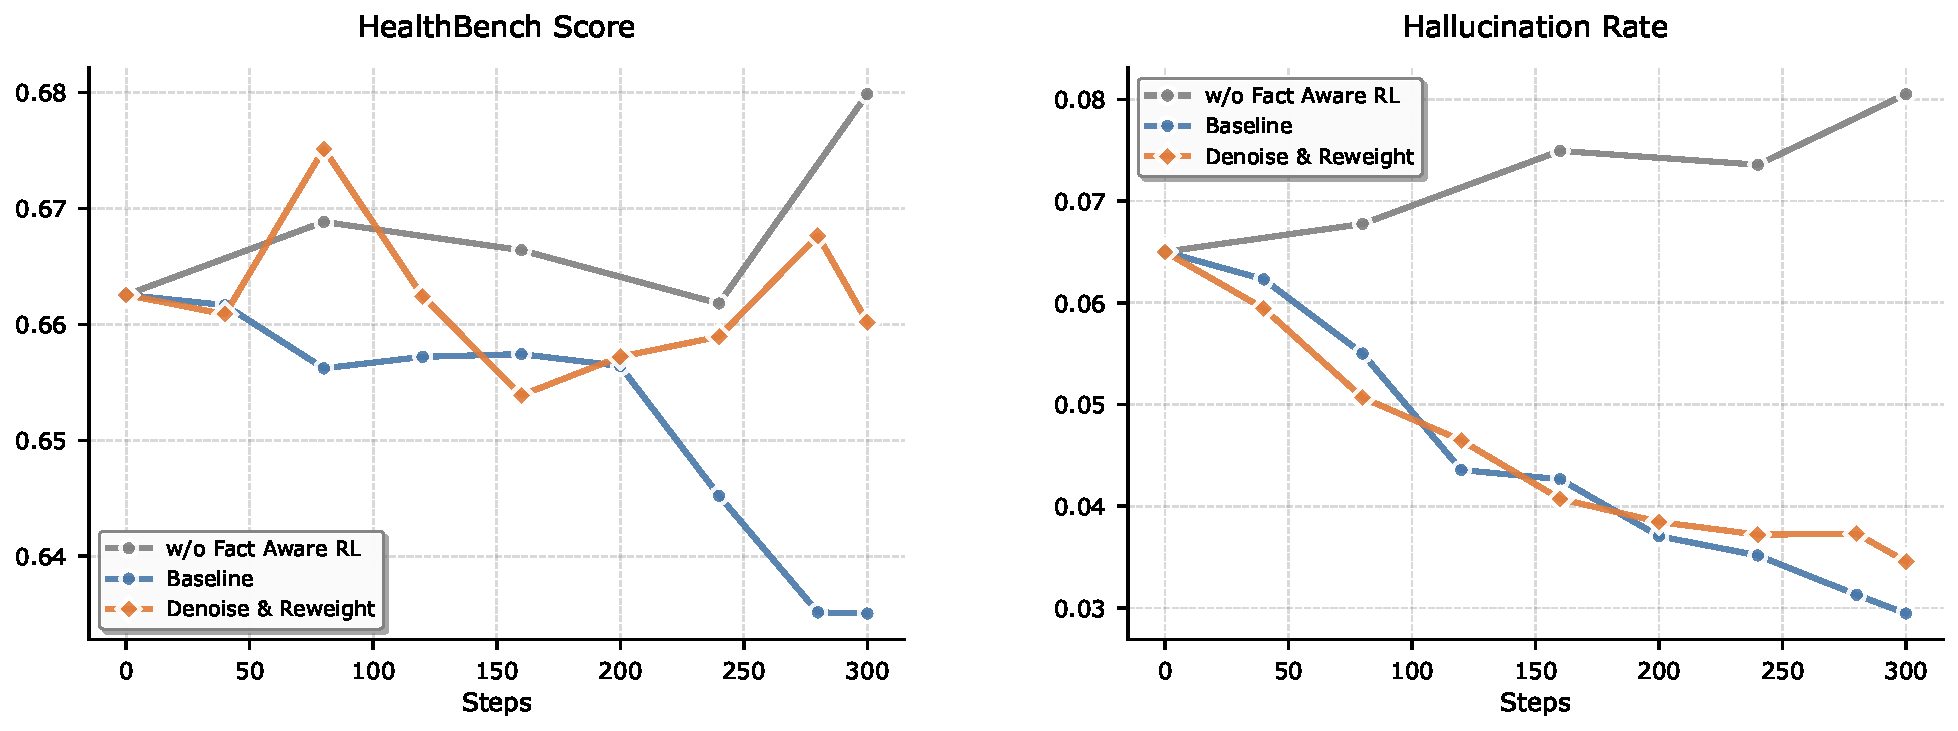
\includegraphics[width=0.98\linewidth]{image/fact-aware-rl-ablation.pdf}
    \caption{不同优化策略的训练动态。图中对比各目标对医学推理能力（左）与事实可靠性（右）的影响。}
    \label{fig:training_dynamics}
\end{figure}

图 \ref{fig:training_dynamics} 展示了不同目标驱动的行为差异。\textit{w/o Fact Aware RL}（灰色）取得最高 HealthBench 得分（约 0.68），但出现明显幻觉漂移（上升到 0.08）。这说明不受约束的优化目标倾向于推动模型生成更长内容，从而削弱事实稳定性。\textit{Baseline}（蓝色）虽纠正了漂移，却过度补偿；其激进的幻觉抑制导致推理能力严重退化，体现惩罚诱导的保守性。

我们在式~\eqref{eq:full-fact-aware-rl} 中提出的 \textit{去噪与重加权} 策略有效将安全对齐与能力损失解耦：其幻觉率降低到约 0.035，与 Baseline 相当，同时推理得分（约 0.665）接近无约束模型起点。这一稳定性验证了双重保护设计的有效性，即边际噪声过滤与能力门控协同工作。因此，该方法在保持核心医学效用的同时，引导模型走向事实正确性。

\subsection{离线专家融合中 Clip-Forward-KL 的消融}
\label{sec:ablation_clip_fkl}

我们分析 Clip-Forward-KL 在离线专家融合中的作用。
学生模型从\textit{医学问诊专家}初始化，并通过离线蒸馏融合\textit{健康咨询专家}。
在相同初始化、数据集与训练配置下，问诊与健康咨询数据分别采用 Clip-Forward-KL 或标准 Forward-KL 进行蒸馏。

表~\ref{tab:clip_ablation} 报告了 ScanBench、HealthBench 与 HealthBench-Hard 的结果。
ScanBench 主要反映医学问诊能力的保留，
而 HealthBench 与 HealthBench-Hard 评估更广泛医疗知识的融合效果。

\begin{table}[H]
\centering
\caption{离线专家融合中 Clip-Forward-KL 的消融。
在相同训练配置下，Clip-Forward-KL 提升 HealthBench 与 HealthBench-Hard，同时保持与 ScanBench 相当的性能。}
\label{tab:clip_ablation}
\begin{tabular}{lccc}
\toprule
Method & ScanBench & HealthBench & HealthBench-Hard \\
\midrule
Forward-KL & 73.7 & 58.6 & 33.2 \\
Clip-Forward-KL & 73.5 & \textbf{61.1} & \textbf{38.5} \\
\bottomrule
\end{tabular}
\end{table}

Clip-Forward-KL 在保持问诊性能的同时显著提升医疗基准，表明其更有效地融合了新领域知识。
这说明标准 Forward-KL 往往会在稀疏离线样本上过度放大概率，从而干扰新医疗能力的融合而非保留既有问诊能力。
通过对教师支持动作施加单侧下界约束，Clip-Forward-KL 实现更保守的融合，并为在线优化提供良好初始化。

\subsection{Gated Eagle-3 推测解码的消融实验}

为保证严格且公平的比较，我们在相同的 35,000 条训练样本与训练协议下，对原始 Eagle-3 草案模型与我们提出的 Gated Eagle-3 进行评估。两者在统一推理配置下覆盖 GSM8K~\cite{DBLP:journals/corr/abs-2110-14168}、HumanEval~\cite{DBLP:journals/corr/abs-2107-03374}、MT-Bench~\cite{DBLP:conf/nips/ZhengC00WZL0LXZ23} 和 HealthBench 等代表性基准。所有实验在 NVIDIA H20 GPU 上进行，模型训练使用 SpecForge~\cite{specforge2025} 框架，推理通过 SGLang~\cite{zheng2024sglang} 执行。如表~\ref{tab:eagle_comparison} 所示，Gated Eagle-3 相比 Eagle-3 基线的平均接受长度提升 0.31。
此外，在并行度为 8 的设置下，吞吐对比如表~\ref{app:eagle_throughput_comparison} 所示。

\label{app:eagle_3}
\begin{table}[H]
\centering
\caption{Eagle-3 基线与 Gated Eagle-3 的平均接受长度对比。}
\label{tab:eagle_comparison}
\begin{tabular}{lcccc}
\toprule
Method & GSM8K & HumanEval & MT-Bench & HealthBench  \\
\midrule
Eagle-3 Base & 3.59 & 3.58 & 2.97 & 2.41 \\
Gated Eagle-3  & \textbf{3.84} & \textbf{4.03} & \textbf{3.23} & \textbf{2.70}  \\
\midrule
$\Delta$ (Gain) & +0.25 & +0.45 & +0.26 & +0.29  \\
\bottomrule
\end{tabular}
\end{table}

\begin{table}[H]
\centering
\caption{Eagle-3 基线与 Gated Eagle-3 的吞吐对比（tokens/s）。}
\label{app:eagle_throughput_comparison}
\begin{tabular}{lcccc}
\toprule
Method & GSM8K & HumanEval & MT-Bench & HealthBench  \\
\midrule
Eagle-3 Base & 376.98 & 576.19 & 451.39 & 356.94  \\
Gated Eagle-3 & \textbf{431.26} & \textbf{646.17} & \textbf{490.12} & \textbf{400.52}  \\
\midrule
$\Delta$ (Gain) & +14.40\% & +12.15\% & +8.58\% & +12.21\%  \\
\bottomrule
\end{tabular}
\end{table}

